\chapter{Thermal Hydraulics}
\label{ch:thermalHydraulics}

\section{Introduction}
  For reactor design purposes, designs are ultimately constrained by thermal
  properties. Additionally, neutronics properties in the form of cross sections
  and density changes are significantly affected by system temperatures.
  Therefore, to accurately simulate the neutron distribution within the reactor,
  it is necessary to also simulate temperatures within the reactor.

  In this simulation, two thermal hydraulic models are
  employed. The first is a one-dimensional fluid flow model to calculate coolant
  temperatures as the coolant flows through a channel. This model is valid for
  the assumption of no cross-flow between channels and perfect fluid mixing 
  within the flow channel. For use in simulating fast reactors with canned
  assemblies and assembly designs which encourage mixing, these assumptions are
  valid. The second model used is a radial
  pin-conduction model to calculate cladding, sodium bond, and fuel temperatures
  based on the heat conduction equation.

  Thermodynamic properties of reactor materials are required for these models.
  The sodium properties required are the most extensive with density, enthalpy, 
  thermal conductivity, dynamic viscosity, and heat capacity required. The 
  functional forms of these properties in this application are given in 
  \cite{sodiumProp}. Additionally, thermal conductivity values are required for 
  cladding and fuel material. Typical cladding for fast reactor designs is HT9
  stainless steel and a functional form of the conductivity is given in
  \cite{ht9Prop}. Fuel composition is assumed to be of the form U-XZr where
  X is the weight fraction of Zr in the fuel. A typical value for X is 10\%.
  Fuel thermal conductivity is given in \cite{fuelProp}. For the expression of
  fuel thermal conductivity given, the integral of thermal conductivity 
  is unbounded as $T \rightarrow 0$ so thermal conductivity is assumed
  constant below 300 K which is below the melting point of sodium so this
  assumption is valid for reactor applications.

\section{Geometric Description}
  For the purposes of the thermal hydraulics model, geometry is described in
  \fref{fig:radial_model}. This model represents a cylindrical fuel pellet,
  surrounded by sodium bond, enclosed in steel cladding, with sodium coolant
  flowing in the axial direction. The center of the fuel pin is located at
  $r=0$ where $r$ is the radial coordinate. The fuel pellet has radius $R_F$ and
  fuel is located in $r \in [0,R_F)$. Then, bond is located in $r \in (R_F,R_B)$
  and clad is located in $r \in (R_B,R_C]$. The fuel center-line temperature is
  $T_0$ and fuel surface temperature is $T_F$. Bond surface temperature is
  $T_B$ and clad surface temperature is $T_C$. $T_{\infty}$ represents the bulk
  coolant temperature. In this model, heat is generated exclusively in the fuel
  with volumetric heat generation rate $q'''$. 

  In a cross-sectional assembly view, dimensions are presented in
  \fref{fig:pin_model} and \fref{fig:hex_can}. In \fref{fig:hex_can}, $Th_{Box}$
  is the thickness of the assembly box, F2F is the flat-to-flat measurement of
  the outside of the hexagonal can, and Pitch is the distance between the
  center of two pins. In future notation, the quantity ``Pitch'' is also noted
  $S$. Using the geometry described in these figures, the material
  cross-sectional areas are calculated according to the given formulae where
  $N_{pin}$ is the number of pins in the assembly.
  \begin{align}
    A_{total} &= \frac{\sqrt{3}}{2} F2F^2 \\
    A_{can} &= A_{total} - 
      \frac{\sqrt{3}}{2} \left(  F2F - 2 \, Th_{Box} \right) \\
    A_{wrap} &= N_{pin} \frac{\pi}{4} D_{wrap}^2 \\
    A_{clad} &= N_{pin} \pi (R_C^2 - R_B^2) \\
    A_{bond} &= N_{pin} \pi (R_B^2 - R_F^2) \\
    A_{fuel} &= N_{pin} \pi R_F^2 \\
    A_{cool} &= A_{total} - A_{can} - A_{wrap} - A_{clad} - A_{bond} - A_{fuel}
  \end{align}
  Calculating the areas as above allows for calculation of cross-sectional area
  fractions. Assuming constant dimensions within an element in the axial
  direction, these area fractions are equivalent to volume fractions and are
  useful for neutron cross section calculations. Additionally, these formulae
  allow for thermal expansion calculations as the liquid sodium in the bond and
  the coolant are allowed to vary to allow for the expansion of other materials.

  \begin{figure}
    \centering
    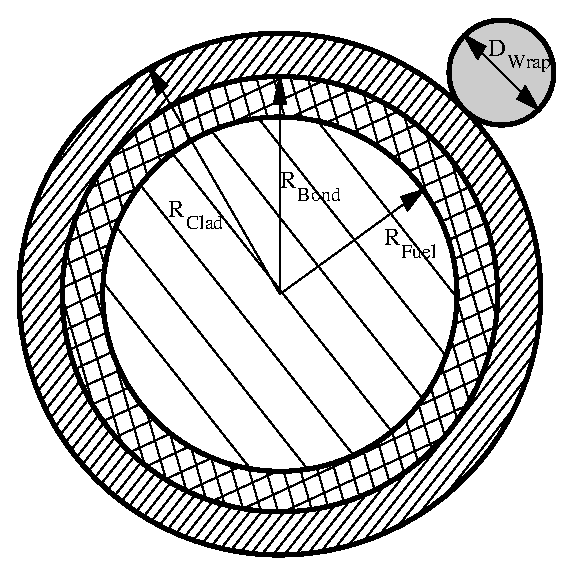
\includegraphics[width=0.5\textwidth]{pin_model}
    \caption{Dimensions of Thermal Hydraulic Pin Model.}
    \label{fig:pin_model}
  \end{figure}

  \begin{figure}
    \centering
    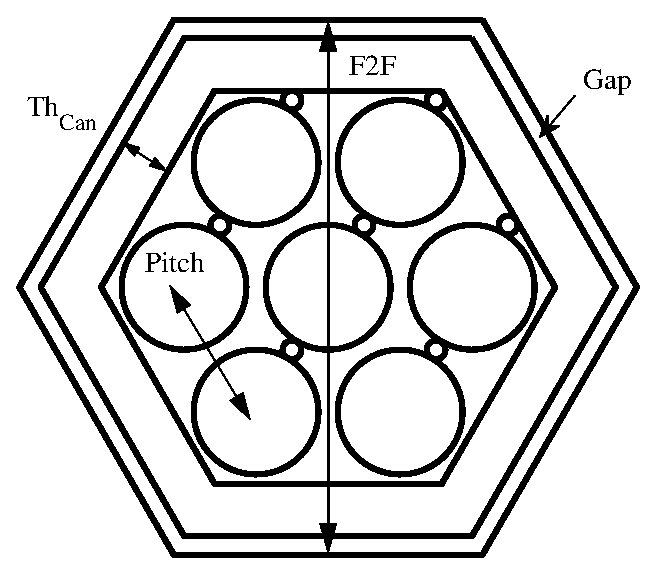
\includegraphics[width=0.5\textwidth]{hex_can}
    \caption{Dimensions of Hexagonal Can.}
    \label{fig:hex_can}
  \end{figure}
  
  \begin{figure}
    \centering
    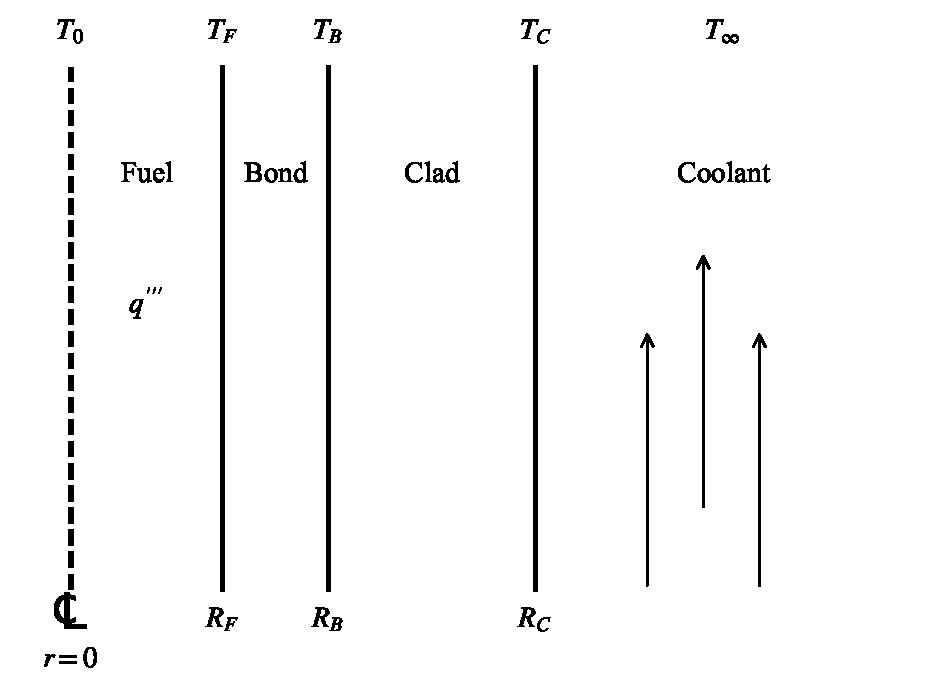
\includegraphics[width=0.5\textwidth]{radial_model}
    \caption{Geometry Description for Thermal Hydraulics Model.}
    \label{fig:radial_model}
  \end{figure}

  Used in association with an unstructured mesh, the thermal hydraulic model
  requires mapping mesh elements to flow channels. For the model described here,
  a flow channel is a single fuel assembly. In the user input to the
  program, the user must specify to which one-dimensional flow channel belongs.
  Adopting the nomenclature from fast reactors, each flow channel represents a
  hexagonal-assembly or a ``hex''. In the following discussion, a hex index is
  subscripted $h$ for $h = 1,2,\ldots,N_h$ where $N_h$ is the number of
  hexagonal assemblies in a reactor. Though the term ``hex'' is used, there is
  no assumption made in any of the calculations that the assembly is indeed
  hexagonal. Square one-dimensional assemblies would be simulated similarly.

  The concept of ``chunks'' is also introduced to aid in the discretization of
  the thermal hydraulic model. A chunk is the set of all elements in a channel
  with a unique axial elevation. For example, in a fast reactor hexagonal
  assembly, the assembly has a unique $h$ index and contains a number of chunks
  equal to the number of axial elevations in the simulation. Additionally, each 
  chunk is required to have unique material composition. The concept of chunks
  is shown in \fref{fig:chunk_description}.  Chunks are indexed
  $c = 1,2,\ldots,N_c$ where $N_c$ is the total number of chunks. For $N_z$
  axial elevations, $N_c = N_h \, N_z$. The indexing
  of chunks is chosen such that $c+N_h$ is the chunk one axial elevation above
  chunk $c$. 

  \begin{figure}
    \centering
    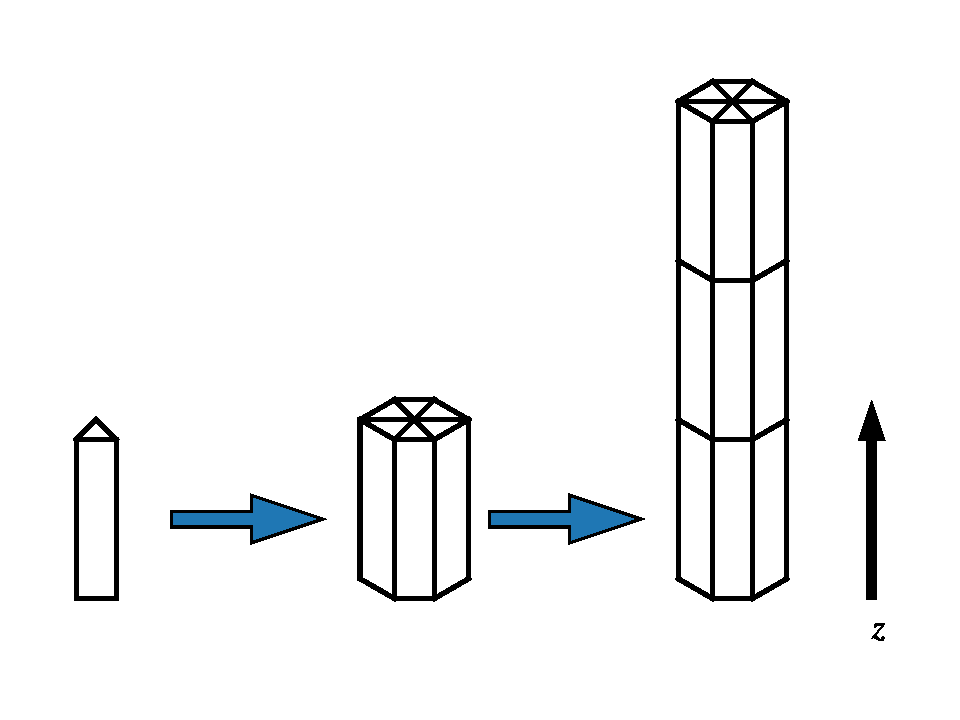
\includegraphics[width=0.7\textwidth]{chunk_description}
    \caption{Progression of Element (left), to Chunk (center), to Hex (right).}
    \label{fig:chunk_description}
  \end{figure}

\section{Power Calculation}
  Recall the multigroup neutron diffusion equation solved via the power
  iteration method returns the largest eigenvalue $\keff$ and unique positive
  eigenvector $\phi_g$ (see \sref{sec:power_iterations}). The flux calculated
  according to this method can be normalized to an arbitrary constant. For a
  specified total reactor power, $Q_{Rx}$ the normalization constant can be 
  calculated. For un-normalized neutron flux $\widetilde{\phi_{g,e}}$ with group
  $g$ in element $e$, the normalization constant is written as
  \begin{equation}
    \label{eq:normalization_c}
    c = \frac{Q_{Rx}}{\sum_{g}^{G} \sum_{e}^{N_E} \kappa \Sigma_{f,g,e} \,
      \widetilde{\phi_{g,e}}}
  \end{equation}
  where $c$ is the normalization constant. $\kappa$ represents the reclaimable
  (non-neutrino) energy produced per fission such that the quantity $\kappa
  \Sigma_f \phi$ represents the heat generation rate. Then the true reactor
  neutron flux is given as
  \begin{equation}
    \label{eq:normalization_phi}
    \phi_{g,e} = c \, \widetilde{\phi_{g,e}}
  \end{equation}
  and the power distribution is 
  \begin{equation}
    \label{eq:normalization_q}
    q_{e} = \sum_g^G \kappa \Sigma_{f,e,g} \phi_{g,e}.
  \end{equation}
  For an elemental power $q_e$, then the volumetric heat generation rate within
  the fuel is 
  \begin{equation}
    \label{eq:elementqppp_fuel}
    q'''_{e} = \frac{q_e}{V_{fuel,e}}
  \end{equation}
  where $V_{fuel,e}$ is the volume of fuel in element $e$. This will be
  necessary for the radial conduction model.

  For the one-dimensional heat convection model in the axial direction,
  heat generation quantities are needed for chunks instead of elements.
  The quantities required are then the total heat generated in a chunk $q_c$ and
  the average volumetric heat generation rate in the fuel for elements within
  the chunk $q'''_c$. These relationships are given in \eref{eq:chunkpwr} and
  \eref{eq:chunkqppp_fuel} respectively. The notation $e \in c$ implies the
  summation over all elements $e$ within chunk $c$.
  \begin{align}
    \label{eq:chunkpwr}
    q_c = \sum_{e \in c} q_e \\
    \label{eq:chunkqppp_fuel}
    q'''_c = \frac{\sum_{e \in c} q'''_e V_{fuel,e}}{\sum_{e \in c} V_{fuel,e}}
  \end{align}

\section{Axial Convection Model}
  \label{sec:axial_convection_model}
  First, the channel mass flow $\mdot_h$ must be calculated for a user specified
  total reactor mass flow rate $\mdot_{Rx}$.  Mass flow is partitioned into each
  channel assuming constant mass flux at the reactor inlet according to 
  \begin{equation}
    \label{eq:mass_flow_split}
    \mdot_h = \mdot_{Rx} \frac{A_{cool,h}}{A_{cool,Rx}}
  \end{equation}
  where $A_{cool,h}$ is the coolant flow area for channel $h$ and $A_{cool,Rx}$
  is the coolant flow area for the reactor.  That is, the mass 
  flow per unit area is assumed constant at the reactor inlet and the mass flow 
  in a channel is the product of the mass flux and the channel flow area. 
  
  The coolant enthalpy for an axial location $z$ within the channel is expressed
  by a simple heat balance equation as
  \begin{equation}
    \label{eq:continuous_heat_balance}
    h_h(x) = h_{in} + \frac{1}{\mdot_h} \int_0^z q'_h(z') \; dz'
  \end{equation}
  where $h$ is the specific enthalpy, $h_{in}$ is the inlet enthalpy, $\mdot_h$
  is the mass flow rate within the channel, and $q'_h(x)$ is the linear heat 
  generation rate for channel $h$ at elevation $z$. $h_{in}$ is related to a
  user specified 
  $T_{inlet}$ by a state relationship for the coolant $h_{in} = h(T_{inlet})$.
  The integral in \eref{eq:continuous_heat_balance} can be discretized along the
  channel and converted to a summation.
  \begin{equation}
    \label{eq:heat_balance}
    \widetilde{h_c} = 
      h_{in} + \frac{1}{\mdot_h} \sum_{i}^{N_z} q'_{i,h} \Delta z_{i,h}
  \end{equation}
  where $q'_{i,h}$ is the linear heat generation rate in the chunk located at 
  axial level $i$ in 
  channel $h$ and $\Delta z_{i,h} = z_{i+1,h} - z_{i,h}$. (Note: by indexing
  properly, $c = h + (i-1) \, N_h$.) Recognizing the 
  quantity $q'_{i,h} \Delta z_{i,h}$ is the total heat generated in channel $h$ 
  at axial level $h$, then \eref{eq:heat_balance} can be rewritten.
  \begin{equation}
    \widetilde{h_c} = h_{in} + \frac{1}{\mdot_h} \sum_i^{N_z} q_{i,h}
  \end{equation}
  The quantity $\widetilde{h_c}$ represents the enthalpy in channel $h$ at axial
  elevation $z_i$. Note that $z_i$ is the upper coordinate of the
  one-dimensional heat convection node. The node-average enthalpy is instead
  desired. To first-order approximation, then
  \begin{equation}
    h_c = \half (\widetilde{h_{i-1,h}} + \widetilde{h_{i,h}})
  \end{equation}
  where $h_c$ is the average enthalpy in chunk $c$ located in channel $h$ at
  axial level $i$.
  The final result of this model is $h_c$, the bulk coolant enthalpy in each
  chunk $c$. Given, $h_c$, bulk coolant temperature $T_{\infty,c} = T(h_c)$ can
  be calculated using a state relationship. This will be an input into the 
  Radial Conduction Model, \sref{sec:radial_conduction_model}, to later 
  calculate the average material temperatures.
  
\section{Radial Conduction Model}
  \label{sec:radial_conduction_model}
  \subsection{Surface Temperature and Center-Line Temperatures}
    \subsubsection{Fuel Center-Line Temperature}
      The fueled region is the only region modeled with non-zero volumetric heat
      generation. In this region, $q'''_c$ as specified by 
      \eref{eq:chunkqppp_fuel} is assumed constant within the fuel. 
      Additionally, the thermal conductivity in the fuel will be assumed to have
      general form $k_F(T)$. For this application, $k_F(T)$ is specified by the
      functional form in \cite{fuelProp} assuming 10\% Zr by weight included in
      fuel.

      The steady-state heat conduction equation with constant volumetric heat
      generation rate $q'''_c$ and variable thermal conductivity $k_F(T)$ can be
      written.
      \begin{equation}
        \label{eq:conduction_fuel}
        \grad \cdot (k_F(T) \grad T_F(r)) + q'''_c = 0
      \end{equation}
      Noting the gradient operator in cylindrical geometry,
      \eref{eq:conduction_fuel} is rewritten with partial derivatives.
      \begin{equation}
        \label{eq:conduction_fuel_cylindrical}
        \frac{1}{r} \frac{\partial}{\partial r} \left( r \, k_F(T) \, 
          \frac{d \, T_F}{dr} \right) + q'''_c = 0
      \end{equation}
      Note the inner derivative is an ordinary derivative because the only
      function to which it applies, $T_F(r)$, is a function of one variable. The
      outer derivative is a partial derivative because it applies to $T_F(r)$ as
      well as $k_F(T) = k_F(T_F(r))$.

      Begin solving \eref{eq:conduction_fuel_cylindrical} by multiplying the
      equation by radial coordinate $r$.
      \begin{equation}
        \frac{\partial}{\partial r} \left( k_F(T_F(r)) \, \frac{d\, T_F}{dr} 
        \right) + q'''_c = 0
      \end{equation}
      Integrate the equation for $r \in [0,r']$ where $r'$ is an arbitrary
      location $r' \in [0,R_F]$.
      \begin{align}
        \int_0^{r'} \left( \frac{\partial}{\partial r} \left( k_F(T_F(r)) \, 
          \frac{d\, T_F}{dr} \right) + q'''_c \right) \; dr &= 0 \\
        \int_0^{r'} \frac{\partial}{\partial r} \left( k_F(T_F(r)) 
          \frac{d \, T_F}{dr} \right) \; dr + \int_0^{r'} q'''_c \; dr &= 0 \\
        \left. r \, k_F(T_F(r)) \frac{d\,T_F}{dr} \right|_{r=0}^{r=r'} + 
          \left. \frac{q'''_c}{2} r^2 \right|_{r=0}^{r=r'} &= 0 \\
        \label{eq:dtdr_fuel}
        \left. r' k_F(T_F(r')) \frac{d\,T_F}{dr} \right|_{r=r'} + 
          \frac{q'''_c}{2} r^{\prime 2} &= 0
      \end{align}
      Divide by the location $r'$.
      \begin{equation}
        \left. k_F(T_F(r')) \frac{d \, T_F}{dr}\right|_{r=r'} + 
          \frac{q'''_c}{2} r' = 0
      \end{equation}
      Next, integrate $r' \in [0,r]$.
      \begin{align}
        \int_0^r \left( k_F(T_F(r')) \left. \frac{d\,T_F}{dr}\right|_{r=r'} 
          + \frac{q'''_c}{2} r' \right) \; dr' &= 0 \\
        \int_0^r k_F(T_F(r')) \left. \frac{d\,T_F}{dr}\right|_{r=r'} \; dr' + 
          \int_0^r \frac{q'''_c}{2} r' \; dr' &= 0 \\
        \int_0^r k_F(T_F(r')) \left. \frac{d\,T_F}{dr}\right|_{r=r'} \; dr' + 
          \left. \frac{q'''_c}{4} r^{\prime 2} \right|_{r'=0}^{r'=r} &= 0 \\
        \int_0^r k_F(T_F(r')) \left. \frac{d\,T_F}{dr}\right|_{r=r'} \; dr' + 
          \frac{q'''_c}{4} r^2 &= 0
      \end{align}
      The fundamental theorem of calculus allows for the expression of the first
      integral.
      \begin{equation}
        \label{eq:tcl_integral}
        \int_{T_F(0)}^{T_F(r)} k_F(T_F(r)) \; dr + \frac{q'''_c}{4} r^2 = 0
      \end{equation}
      In this derivation, $k_F(T)$ is allowed to be a generic function. 
      Therefore, \eref{eq:tcl_integral} does not have a simple forward 
      expression. Solving for $T_F(0)$ will require a non-linear search such as
      the bisection method. Define the conductivity integral of the generic
      conductivity function $k(T)$ as
      \begin{equation}
        \label{eq:conductivity_integral}
        K(T) = \int_0^T k(T') \; dT'.
      \end{equation}
      Then, \eref{eq:tcl_integral} can be rewritten.
      \begin{gather}
        K_F(T_F(r)) - K_F(T_F(0)) + \frac{q'''_c}{4} r^2 = 0 \\
        K_F(T_F(0)) = K_F(T_F(r)) + \frac{q'''_c}{4} r^2 \\
        \label{eq:tcl_conductivity_integral}
        K_F(T_F(0)) = K_F(T_F) + \frac{q'''_c}{4} R_F^2
      \end{gather}
      The fuel center-line temperature can be calculated using
      \eref{eq:tcl_conductivity_integral} given a functional form of the
      conductivity integral $K_F(T)$ by performing a search on the function
      where $T_F(0)$ is the fuel center-line temperature, $T_F=T_F(R_F)$ is the
      fuel surface temperature, and $R_F$ is the radius of the fuel. To
      calculate $T_F(0)$, the fuel surface temperature must be known.
      If more information is known about $K_F(T)$, a forward expression
      may be possible. However, a bisection method is implemented to maintain
      generality.

    \subsubsection{Fuel Surface Temperature}
      The fuel surface temperature is calculated by considering the heat
      conduction equation in the sodium bond region. There is no heat generation
      in this region so $q'''=0$.
      The steady-state heat conduction equation with no heat generation is
      written as
      \begin{equation}
        \label{eq:tc_grad}
        \grad \cdot (k_B(T_B(r)) \grad T_B(r)) = 0
      \end{equation}
      where $k_B(T)$ is a general expression for the thermal conductivity in the
      sodium bond and is given by a state relationship in \cite{sodiumProp}.
      $T_B(r)$ is the temperature within the cladding region.
      In this region, good thermal contact is
      assumed such that $T_F(R_F)=T_B(R_F)$. That is, the temperature is 
      continuous at the material discontinuity. Additionally, constant heat flux
      is assumed at the material discontinuity such that $k_F(T_F(R_F))
      \left.\frac{d\,T_F}{dr}\right|_{r=R_F} = k_B(T_B(R_F))
      \left.\frac{d\,T_B}{dr}\right|_{r=R_F}$.

      Recognizing cylindrical geometry, \eref{eq:tc_grad} can be rewritten.
      \begin{equation}
        \label{eq:tb_heat_conduction}
        \frac{1}{r} \frac{\partial}{\partial r} \left(
          r \, k_B(T_B(r)) \frac{d \, T_B}{dr} \right) = 0
      \end{equation}
      Begin solving \eref{eq:tb_heat_conduction} by multiplying the equation by
      the radial coordinate $r$.
      \begin{equation}
        \frac{\partial}{\partial r} \left( r \, k_B(T_B(r)) \frac{d \, T_B}{dr}
          \right) = 0
      \end{equation}
      Integrate the equation for $r \in[R_F,r']$ where $r'$ is an arbitrary
      location $r' \in [R_F,R_B]$.
      \begin{align}
        \int_{R_F}^{r'} \frac{\partial}{\partial r} \left( r\, k_B(T_B(r)) \, 
          \frac{d\,T_B}{dr} \right) \; dr &= 0\\
        \left. r\, k_B(T_B(r)) \frac{d\,T_B}{dr} \right|_{r=R_F}^{r=r'} &= 0 \\
        \label{eq:tf_first_integral}
        \left. r' \, k_B(T_B(r')) \frac{d\,T_B}{dr} \right|_{r=r'} - 
          \left. R_F \, k_B(T_B(R_F)) \frac{d\,T_B}{dr} \right|_{r=R_F} &= 0
      \end{align}
      The assumption of constant heat flux allows for the treatment of the
      spatial derivative at $R_F$. Recall from the derivation within the fuel
      region, the expression \eref{eq:dtdr_fuel} is exploited. The expression is
      valid for any $r' \in [0,R_F]$ so allow $r'=R_F$.
      \begin{align}
        \left. R_F k_F(T_F(R_F)) \frac{d\,T_F}{dr} \right|_{r=R_F} + 
          \frac{q'''_c}{2} R_F^2 &= 0 \\
        \label{eq:surface_relation}
        \left. R_F k_F(T_F(R_F)) \frac{d\,T_F}{dr} \right|_{r=R_F} &= 
          - \frac{q'''_c}{2} R_F^2
      \end{align}
      Recall from the earlier derivation that the quantity $q'''_c$ is the
      average volumetric heat generation rate within chunk $c$.
      \eref{eq:surface_relation} is substituted into
      \eref{eq:tf_first_integral}.
      \begin{equation}
        \label{eq:tf_first_bc}
        \left. r' \, k_B(T_B(r')) \frac{d\,T_B}{dr} \right|_{r=r'} +
          \frac{q'''_c}{2} R_F^2 = 0
      \end{equation}
      Divide \eref{eq:tf_first_integral} by the radial coordinate $r'$. This is
      valid because $r \ne 0$ in this region.
      \begin{equation}
        \left. k_B(T_B(r')) \frac{d\,T_B}{dr} \right|_{r=r'} + 
          \frac{q'''_c}{2} \frac{R_F^2}{r'} = 0
      \end{equation}
      Integrate the equation for $r' \in [R_F,r]$ where $r \in [R_F,r']$.
      \begin{align}
        \int_{R_F}^r \left( \left. k_B(T_B(r')) \frac{d\,T_B}{dr}\right|_{r=r'}
          + \frac{q'''_c}{2} \frac{R_F^2}{r'} \right) \; dr' &= 0 \\
        \int_{R_F}^r \left. k_B(T_B(r')) \frac{d\,T_B}{dr}\right|_{r=r'} \; dr'
          + \int_{R_F}^r \frac{q'''_c}{2} \frac{R_F^2}{r'} \; dr' &= 0\\
        \int_{R_F}^r \left. k_B(T_B(r')) \frac{d\,T_B}{dr}\right|_{r=r'} \; dr'
          + \frac{q'''_c}{2} R_F^2 \left. \ln(r') \right|_{r'=R_F}^{r'=r} &= 0\\
        \int_{R_F}^r \left. k_B(T_B(r')) \frac{d\,T_B}{dr}\right|_{r=r'} \; dr'
          + \frac{q'''_c}{2} R_F^2 ( \ln(r) - \ln(R_F)) &= 0 \\
        \int_{R_F}^r \left. k_B(T_B(r')) \frac{d\,T_B}{dr}\right|_{r=r'} \; dr'
          + \frac{q'''_c}{2} R_F^2 \ln\left(\frac{r}{R_F}\right) &= 0 
      \end{align}
      Again, the remaining integral can be rewritten by employing the
      fundamental theorem of calculus.
      \begin{equation}
        \label{eq:tf_fundamental_theorem}
        \int_{T_B(R_F)}^{T(r)} k_B(T_B(r)) \; dT + \frac{q'''_c}{2} R_F^2 
          \ln\left(\frac{r}{R_F}\right) = 0
      \end{equation}
      Defining a conductivity integral function $K_B(T)$ similar to
      \eref{eq:conductivity_integral}, \eref{eq:tf_fundamental_theorem} can be
      rewritten.
      \begin{gather}
        K_B(T_B(r)) - K_B(T_B(R_F)) + \frac{q'''_c}{2} R_F^2
          \ln\left(\frac{r}{R_F}\right) = 0 \\
        K_B(T_B(R_F)) = K_B(T_C(r)) + \frac{q'''_c}{2} R_F^2
          \ln\left(\frac{r}{R_F}\right) \\
        \label{eq:tf_conductivity_integral}
        K_B(T_F) = K_B(T_B) + \frac{q'''_c}{2} R_F^2
          \ln\left(\frac{R_B}{R_F}\right)
      \end{gather}
      The fuel surface temperature can be calculated using
      \eref{eq:tf_conductivity_integral} given a functional form of the
      conductivity integral $K_B(T)$ by performing a search on the function. In
      \eref{eq:tf_conductivity_integral}, $T_F=T_B(R_F)$ is the fuel surface 
      temperature, $T_B=T_B(R_B)$ is the bond surface temperature and must be
      given to use this expression.

    \subsubsection{Bond Surface Temperature}
      Consider the heat conduction equation in the cladding region. Derivation
      of the bond surface temperature $T_B=T_B(R_B)$ is similar to
      the fuel surface temperature because both consider a heat conduction
      equation with no heat generation. The steady-state heat conduction 
      equation for this region is written as
      \begin{equation}
        \label{eq:clad_conduction_grad}
        \grad \cdot (k_C(T_C(r)) \grad T_C(r)) = 0
      \end{equation}
      where $k_C(T)$ is a functional form of the thermal conductivity in the
      cladding from \cite{ht9Prop}. $T_C(r)$ is the temperature within the
      cladding region and $T_C=T_C(R_C)$ is the cladding surface temperature. 
      In this region, good thermal contact is assumed such that
      $T_B(R_B)=T_C(R_B)$. Additionally, constant heat flux is assumed at the
      cladding-bond boundary such that $\left. k_B(T_B(R_C))
      \frac{d\,T_B}{dr}\right|_{r=R_C} = \left. k_C(T_C(R_C))
      \frac{d\,T_C}{dr}\right|_{r=R_F}$.

      Rewriting the gradient for cylindrical geometry,
      \eref{eq:clad_conduction_grad}.
      \begin{equation}
        \label{eq:clad_conduction}
        \frac{1}{r} \frac{\partial}{\partial r} \left( r\, k_C(T_C(r)) 
          \frac{d\,T_C}{dr} \right) = 0
      \end{equation}
      Begin solving \eref{eq:clad_conduction} by multiplying the equation by the
      radial coordinate $r$.
      \begin{equation}
        \frac{\partial}{\partial r} \left( r\,k_C(T_C(r))\,\frac{d\,T_C}{dr}
          \right) = 0
      \end{equation}
      Integrate the equation through $r \in [R_B,r']$ where $r'$ is an arbitrary
      coordinate $r' \in [R_B,R_C]$.
      \begin{align}
        \int_{R_B}^{r'} \frac{\partial}{\partial r} \left( r \, k_C(T_C(r))
          \frac{d\,T_C}{dr} \right) \; dr &= 0 \\
        \left. r\,k_C(T_C(r)) \frac{d\,T_C}{dr} \right|_{r=R_B}^{r=r'} &= 0 \\
        \label{eq:clad_before}
        \left. r' \, k_C(T_C(r')) \frac{d\,T_C}{dr} \right|_{r=r'} - 
          \left. R_B \, k_C(T_C(R_B)) \frac{d\,T_C}{dr} \right|_{r=R_B} &= 0
      \end{align}
      The assumption of constant heat flux at the material discontinuity at
      $R_B$ allows for an expression of the derivative at $R_B$. Recall from the
      derivation within the bond region, the expression \eref{eq:tf_first_bc}
      can be used. The expression is valid for any $r' \in [R_F,R_B]$ so allow
      $r'=R_B$.
      \begin{align}
        \left. R_B \, k_B(T_B(R_B)) \frac{d\,T_B}{dr} \right|_{r=R_B} +
          \frac{q'''_c}{2} R_F^2 &= 0 \\
        \label{eq:clad_bc_relation}
        \left. R_B \, k_B(T_B(R_B)) \frac{d\,T_B}{dr} \right|_{r=R_B} &= 
          - \frac{q'''_c}{2} R_F^2
      \end{align}
      Recalling again that $q'''_c$ is the average volumetric heat generation
      rate in the fuel within chunk $c$. \eref{eq:clad_bc_relation} is
      inserted into \eref{eq:clad_before}.
      \begin{equation}
        \left. r' \, k_C(T_C(r')) \frac{d\,T_C}{dr} \right|_{r=r'} + 
          \frac{q'''_c}{2} R_F^2 = 0
      \end{equation}
      Divide by $r'$ because $r' \ne 0$ in this region.
      \begin{equation}
        \left. k_C(T_C(r')) \frac{d\,T_C}{dr} \right|_{r=r'} + 
          \frac{q'''_c}{2} \frac{R_F^2}{r'} = 0
      \end{equation}
      Integrate the equation for $r' \in [R_B,r]$ where $r \in [R_B,r']$.
      \begin{align}
        \int_{R_B}^r \left( \left. k_C(T_C(r')) \frac{d\,T_C}{dr} \right|_{r=r'}
          + \frac{q'''_c}{2} \frac{R_F^2}{r'} \right) \; dr' &= 0 \\
        \int_{R_B}^r \left. k_C(T_C(r')) \frac{d\,T_C}{dr} \right|_{r=r'} \; dr'
          + \int_{R_B}^r \frac{q'''_c}{2} \frac{R_F^2}{r'} \; dr' &= 0 \\
        \int_{R_B}^r \left. k_C(T_C(r')) \frac{d\,T_C}{dr} \right|_{r=r'} \; dr'
          + \frac{q'''_c}{2} R_F^2 \left. \ln(r') \right|_{r'=R_B}^{r'=r} &= 0\\
        \int_{R_B}^r \left. k_C(T_C(r')) \frac{d\,T_C}{dr} \right|_{r=r'} \; dr'
          + \frac{q'''_c}{2} R_F^2 (\ln(r) - \ln(R_B)) &= 0\\
        \int_{R_B}^r \left. k_C(T_C(r')) \frac{d\,T_C}{dr} \right|_{r=r'} \; dr'
          + \frac{q'''_c}{2} R_F^2 \ln\left(\frac{r}{R_B}\right) &= 0
      \end{align}
      Again, the integral term can be rewritten with use of the fundamental
      theorem of calculus.
      \begin{equation}
        \label{eq:clad_integral}
        \int_{T_C(R_B)}^{T_C(r)} k_C(T_C(r)) \; dr +
          \frac{q'''_c}{2} R_F^2 \ln\left(\frac{r}{R_B}\right) = 0
      \end{equation}
      Defining a conductivity integral function $K_C(T)$ similar to
      \eref{eq:conductivity_integral}, \eref{eq:clad_integral} can be rewritten.
      \begin{gather}
        K_C(T_C(r)) - K_C(T_C(R_B)) + \frac{q'''_C}{2} R_F^2
          \ln\left(\frac{r}{R_B}\right) = 0 \\
        K_C(T_C(R_B)) = K_C(T_C(r)) + \frac{q'''_c}{2} R_F^2
          \ln\left(\frac{r}{R_B}\right) \\
        \label{eq:ktb}
        K_C(T_B) = K_C(T_C) + \frac{q'''_C}{2} R_F^2
          \ln\left(\frac{R_C}{R_B}\right) 
      \end{gather}
      The bond surface temperature can be calculated using \eref{eq:ktb} given a
      function describing the cladding conductivity integral $K_C(T)$ and
      performing a bisection method search on the function. In \eref{eq:ktb},
      $T_B = T_C(R_B)$ is the bond surface temperature, $T_C=T_C(R_C)$ is the
      clad surface temperature and is calculated using a different method and
      treated as an input to this method.  

    \subsubsection{Clad Surface Temperature}
      Clad surface temperature $T_C$ is given by Newton's Law of Cooling with
      convective heat transfer coefficient $h_c$ specified according to the
      Weisman Correlation. Newton's Law of Cooling may be written as
      \begin{equation}
        q''_{clad} = h_c (T_C - T_{\infty})
      \end{equation}
      where $q''_{clad}$ is the heat flux at the clad surface $R_C$, $h_c$ is
      the convective heat transfer coefficient, $T_C$ is the clad surface
      temperature, and $T_{\infty}$ is the bulk coolant temperature. Using the
      relationships in \sref{sec:axial_convection_model}, $T_{\infty}$ is given
      by the state relationship $T_{\infty} = T(h_c)$. The heat flux at the clad
      surface is related to the volumetric heat generation rate in the fuel
      according to 
      \begin{equation}
        q''_{clad} = q'''_c \frac{R_F^2}{2 R_C}
      \end{equation}
      where $q'''_c$ is the chunk-average volumetric heat generation rate in the
      fuel according to \eref{eq:chunkqppp_fuel}.

      The coefficient $h_c$ must be calculated via an applicable correlation.
      The Weisman correlation is selected because it is valid for general fluid
      flow and has parameters correlated for triangular pitch flow areas common
      to fast reactor designs. The Weisman Correlation relates the Nusselt,
      Reynolds, and Prandlt dimensionless numbers according to
      \begin{equation}
        \label{eq:weisman}
        Nu = C \, Re^{0.8} \, Pr^{1/3}
      \end{equation}
      where $Nu$ is the Nusselt number, $Re$ is the Reynolds number, $Pr$ is 
      the Prandlt number, and $C$ is a correlation coefficient specified by the
      triangular geometry. For triangular pitch flow, the geometry is described
      as
      \begin{align}
        \label{eq:weisman_c}
        C &= 0.026 \frac{S}{2 \, R_C} - 0.006 \\
        \label{eq:weisman_ax}
        A_x &= \frac{\sqrt{3}}{4} S^2 - \frac{\pi R_C^2}{2} \\
        \label{eq:weisman_pw}
        P_w &= \pi R_C \\
        \label{eq:weisman_de}
        D_e &= \frac{4 \, A_x}{P_w}
      \end{align}
      where $S$ is the pitch between pins (see \fref{fig:hex_can}), $A_x$ is the
      flow cross-sectional area, $P_w$ is the flow wetted perimeter, and $D_e$
      is the effective flow diameter. The Reynolds number is defined as
      \begin{equation}
        \label{eq:re}
        Re = \frac{\mdot_h \, D_e}{A_x \, \mu}
      \end{equation}
      where $\mdot_h$ is the assembly mass flow rate, $\mu$ is the fluid's
      dynamic viscosity given by a state relationship, and $D_e$ and $A_x$ are 
      defined according to \eref{eq:weisman_de} and \eref{eq:weisman_ax}
      respectively. The Prandtl number is defined according to 
      \begin{equation}
        \label{eq:pr}
        Pr = \frac{c_p \, \mu}{k}
      \end{equation}
      where $c_p$ is the fluid specific heat capacity at constant pressure, 
      $\mu$ is the fluid dynamic viscosity, and $k$ is the fluid thermal 
      conductivity. Note that each of these quantities are given by state 
      relationships. As such, the Prandtl number can itself be correlated for a
      given fluid as a state relationship.
      
      With the dimensionless quantities expressed in \eref{eq:re} and
      \eref{eq:pr}, the Weisman correlation is used to calculate the Nusselt
      number. Given a Nusselt number, the convective heat transfer coefficient
      is defined as
      \begin{equation}
        \label{eq:hc}
        h_c = \frac{Nu \, k}{D_e}
      \end{equation}
      where $Nu$ is the Nusselt number from the Weisman correlation
      \eref{eq:weisman}, $k$ is the fluid thermal conductivity given by a state
      relationship, and $D_e$ is the effective flow diameter given in
      \eref{eq:weisman_de}. Finally, the clad surface temperature is expressed.
      \begin{align}
        T_C &= \frac{q''_{clad}}{h_c} + T_{\infty} \\
        \label{eq:tc}
        T_C &= q'''_c \frac{R_F^2}{2\,R_c\,h_c} + T_{infty}
      \end{align}

  \subsection{Average Temperatures}
\section{Cross Section Treatment}
  \subsection{Cross Section Library Generation}
  \subsection{Temperature Dependent Cross Section Calculation}

% todo this will probably be a separate chapter and include thermal expansion
%\section{Results}
%  \subsection{Single Pin Model}
%  \subsection{Reactor Simulation}
